% Compile with XeLaTeX.
\documentclass[10pt,a4paper]{article}

\usepackage[a4paper,margin=1.65cm]{geometry}
\usepackage{fontspec}
\IfFileExists{/System/Library/Fonts/Supplemental/Arial.ttf}{
  \setmainfont[
    Path=/System/Library/Fonts/Supplemental/,
    UprightFont={Arial.ttf},
    BoldFont={Arial Bold.ttf},
    ItalicFont={Arial Italic.ttf},
    BoldItalicFont={Arial Bold Italic.ttf}
  ]{Arial}
  \setsansfont[
    Path=/System/Library/Fonts/Supplemental/,
    UprightFont={Arial.ttf},
    BoldFont={Arial Bold.ttf},
    ItalicFont={Arial Italic.ttf},
    BoldItalicFont={Arial Bold Italic.ttf}
  ]{Arial}
}{
  \IfFontExistsTF{Times New Roman}{\setmainfont{Times New Roman}}{\setmainfont{TeX Gyre Termes}}
  \IfFontExistsTF{Arial}{\setsansfont{Arial}}{\setsansfont{TeX Gyre Heros}}
}
\usepackage{graphicx}
\usepackage{booktabs}
\usepackage{tabularx}
\usepackage{array}
\usepackage{enumitem}
\usepackage{xcolor}
\usepackage{hyperref}
\usepackage{caption}
\usepackage{subcaption}
\usepackage{float}
\usepackage{url}
\usepackage{xurl}
\usepackage{amsmath}
\usepackage{longtable}

\graphicspath{{../outputs/figures/}{outputs/figures/}}
\hypersetup{
  colorlinks=true,
  linkcolor=black,
  urlcolor=blue,
  citecolor=black
}

\setlength{\parskip}{4pt}
\setlength{\parindent}{0pt}
\emergencystretch=4em
\setlist[itemize]{leftmargin=1.2em,itemsep=2pt,topsep=2pt}
\setlist[enumerate]{leftmargin=1.4em,itemsep=2pt,topsep=2pt}
\captionsetup{font=small,labelfont=bf}
\renewcommand{\arraystretch}{1.12}
\renewcommand{\contentsname}{Mục lục}
\renewcommand{\figurename}{Hình}
\renewcommand{\tablename}{Bảng}

\newcommand{\TenDeTai}{ODA-based Multi-sensor Risk-aware UAV Obstacle Avoidance Benchmark}
\newcommand{\SinhVien}{Nguyễn Thanh Lâm}
\newcommand{\Mentor}{Hoàng Công Phát}
\newcommand{\DonViMentor}{Viettel High Tech}
\newcommand{\EmailMentor}{}
\newcommand{\code}[1]{\texttt{#1}}

\begin{document}

\begin{center}
{\Large\bfseries \TenDeTai}\\[3pt]
{\large\bfseries Báo cáo tiến độ chi tiết: câu chuyện nghiên cứu và kết quả hiện tại}\\[5pt]
{\normalsize \SinhVien, \Mentor\textsuperscript{1}}\\
{\small \textsuperscript{1}\DonViMentor}\\[4pt]
{\small Bản này là bản dài để báo cáo tiến trình và thảo luận với mentor, không bị ràng buộc bởi giới hạn 6 trang của bản nộp chính thức.}
\end{center}

\vspace{-1mm}
\tableofcontents
\vspace{2mm}

\section{Câu chuyện chính muốn kể với mentor}

Điểm cốt lõi của đề tài không phải là ``em chạy một model depth'' hay ``em vẽ được vài hình''. Câu chuyện mạnh hơn là: từ một dataset UAV có đủ camera, radar, IMU và OptiTrack, sinh viên đã biến nó thành một benchmark tránh vật cản có thể đo được, so sánh được và mở rộng được. Trục kể chuyện nên đi theo bốn lớp.

\textbf{Lớp 1 - Ground truth trước, học máy sau.}
ODA Dataset có MAV bay trong nhà, có vật cản và có OptiTrack ground truth. Vì vậy bước đúng nhất là dựng lại quỹ đạo thật, vị trí vật cản và khoảng cách an toàn trước. Từ đó, mọi kết quả phía sau đều có điểm tựa: biết lúc nào MAV gần vật cản, lúc nào vi phạm safety distance, lúc nào chỉ là cảnh báo giả.

\textbf{Lớp 2 - Planner cho thấy bài toán hình học có thể giải được.}
Khi benchmark 300 trial, các planner cổ điển như A*, RRT, RRT* và MPPI đều tạo được đường tránh vật cản an toàn hơn straight-line và quỹ đạo người lái. Điều này cho thấy phần lập kế hoạch hình học có thể xây dựng được trong một pipeline nhẹ. Nhưng nó cũng đặt ra câu hỏi nghiên cứu sâu hơn: nếu planner có thể tránh được vật cản khi biết ground truth, thì vấn đề thực tế nằm ở perception, độ tin cậy cảm biến và cảnh báo rủi ro sớm.

\textbf{Lớp 3 - Perception-risk là cầu nối từ cảm biến sang an toàn.}
Thay vì chỉ hiển thị RGB/depth đẹp mắt, pipeline biến depth/radar/IMU thành feature theo thời gian và dự đoán future-risk. Kết quả cho thấy bài toán bị mất cân bằng nhãn mạnh: đa số frame là an toàn, frame nguy hiểm ít hơn nhiều. Vì vậy accuracy không đủ; cần macro-F1, balanced accuracy và recall của lớp nguy hiểm. Đây là điểm nói với mentor để chứng minh mình hiểu bản chất đánh giá safety-critical system.

\textbf{Lớp 4 - LiDAR bên ngoài ODA dùng để tăng độ khó perception, không làm loãng benchmark chính.}
ODA vẫn là benchmark chính vì nó đúng bài toán UAV obstacle avoidance. Multi-LiDAR và ARCO được dùng như stress-test cảm biến: đọc point cloud thật, ground removal, voxel clustering và 3D bounding box. Nhánh này hiện đã chạy trên HolybroStdn01, Tello03 và TelloOut02 với ba nguồn point cloud Ouster/Mid360/Avia; vì vậy phần LiDAR không còn là probe metadata mà là một pipeline xử lý point cloud thật. Tuy nhiên metric tránh vật cản UAV vẫn lấy từ ODA để tránh so sánh lẫn lộn giữa các dataset khác bản chất.

\begin{table}[H]
\centering
\small
\caption{Thông điệp ngắn khi trình bày với mentor.}
\begin{tabularx}{0.96\linewidth}{>{\bfseries}p{3.0cm} X}
\toprule
Nếu mentor hỏi & Câu trả lời nên nhấn mạnh \\
\midrule
Em đang làm gì? & Em xây dựng một benchmark UAV obstacle avoidance trên ODA: từ trajectory ground truth, obstacle representation, safety metric, planner comparison đến perception-risk đa cảm biến. \\
Điểm mới ở đâu? & Không chỉ chạy visualization gốc; em tạo pipeline đo risk theo thời gian, so sánh planner, thêm predicted depth, radar, IMU, và có nhánh LiDAR point-cloud segmentation/3D bbox thật để chứng minh khả năng xử lý sensing phức tạp. \\
Tại sao không dùng ROS/Gazebo trước? & Vì mục tiêu hiện tại là kết quả nhanh, tái lập được và kiểm chứng bằng dữ liệu thật. ROS/Gazebo/FAST-LIVO2 là hướng mở rộng, không phải điều kiện để có benchmark ban đầu. \\
Kết quả quan trọng nhất? & 300/300 ODA trial sẵn sàng, 2100 dòng planner metric, 2584 dòng perception-risk feature trên 50 trial, video 6 panel, và Multi-LiDAR HolybroStdn01/Tello03/TelloOut02 có point-cloud segmentation, clustering và 3D bbox thật từ Ouster/Mid360/Avia. \\
Điểm hạn chế hiện tại? & Depth vẫn là relative depth, TensorRT engine thật chưa đo được, smoothness mới là proxy 2D, và LiDAR external chỉ là stress-test chứ chưa phải benchmark UAV chính. \\
\bottomrule
\end{tabularx}
\end{table}

\section{Trạng thái tiến độ hiện tại}

Báo cáo này nên được đọc như một bản tiến độ: mục tiêu chưa phải là ``đóng gói kết quả cuối cùng'', mà là chứng minh dự án đã đi từ demo định tính sang một benchmark có số liệu, có pipeline tái lập và có câu chuyện nghiên cứu rõ ràng. Các kết quả hiện tại có thể chia thành ba cụm:

\begin{enumerate}
  \item \textbf{Benchmark chính trên ODA:} đã mở rộng từ 3 sample ban đầu lên 300 trial, có bảng so sánh human trajectory, straight-line, geometric bypass, A*, RRT, RRT* và MPPI.
  \item \textbf{Perception-risk đa cảm biến:} đã có video 6 panel, Depth Anything V2 Small trên 50 trial, feature depth/radar/IMU, và classifier future-risk có phân tích mất cân bằng nhãn.
  \item \textbf{LiDAR stress-test ngoài ODA:} đã upload/download qua Hugging Face và chạy segmentation/clustering/3D bbox thật trên Multi-LiDAR HolybroStdn01, Tello03 và TelloOut02. Phần này dùng để chứng minh năng lực xử lý LiDAR, còn ODA vẫn là benchmark UAV obstacle-avoidance chính.
\end{enumerate}

\begin{table}[H]
\centering
\small
\caption{Snapshot tiến độ để mở đầu buổi báo cáo với mentor.}
\begin{tabularx}{0.96\linewidth}{>{\bfseries}p{3.7cm} X}
\toprule
Mảng công việc & Trạng thái hiện tại \\
\midrule
ODA data/benchmark & 300/300 trial mục tiêu đã sẵn sàng; 2100 dòng planner metric; 0 planner crash trong batch 300 trial. \\
Planner comparison & A*, RRT, RRT* đạt 0 collision và 0 safety violation trên 300 trial; MPPI có mean clearance cao nhưng compute time lớn hơn RRT/A*. \\
Video định tính & Có video 6 panel: RGB, relative depth, radar FFT, IMU, safety map và trajectory; contact sheet trong bản này đã được xếp dọc để đọc rõ từng panel. \\
Depth/risk & Depth Anything V2 Small chạy 50 trial/2584 frame; bảng perception-risk có split theo trial ID và threshold tuning cho macro-F1/recall. \\
LiDAR thật & Multi-LiDAR HolybroStdn01, Tello03, TelloOut02 đã có segmentation/clustering/3D bbox thật từ Ouster, Mid360 và Avia; kết quả đã lưu trên Hugging Face và local outputs. \\
Điểm chưa claim & Depth chưa phải metric depth; TensorRT engine thật chưa đo; feasibility vẫn là proxy 2D; external LiDAR dùng cho stress-test, không thay ODA. \\
\bottomrule
\end{tabularx}
\end{table}

\section{Bối cảnh và lựa chọn bài toán}

UAV/MAV bay trong nhà thường không có GNSS, không gian hẹp, vật cản có thể xuất hiện gần và thời gian phản ứng ngắn. Nếu chỉ dùng hình ảnh định tính, ta khó trả lời các câu hỏi mentor thường hỏi: đường bay có an toàn không, khoảng cách gần nhất là bao nhiêu, có vượt ngưỡng safety distance không, planner nào tốt hơn, và cảm biến nào giúp cảnh báo rủi ro.

ODA Dataset phù hợp với mục tiêu này vì có đúng cấu trúc cần cho một pipeline nhẹ: RGB camera, event camera, radar 24 GHz, IMU và OptiTrack ground truth \cite{odaGithub,oda4tu,odaPaper}. Trong giai đoạn này, pipeline chủ động tránh ROS/Gazebo và các hệ nặng như FAST-LIVO2 để tập trung vào thứ có thể kiểm chứng ngay: CSV/metadata, trajectory, obstacle coordinates, hình ảnh/video và metric.

\begin{figure}[H]
\centering
\includegraphics[width=0.98\linewidth]{qualitative_depth_sensor_sample_3_contact_sheet_vertical.png}
\caption{Một kết quả định tính tiêu biểu cho trial 3, xếp dọc bốn thời điểm để từng panel dễ đọc hơn: RGB, relative monocular depth, radar FFT, IMU, safety map và trajectory. Đây là case MAV không collision trực tiếp nhưng đi vào vùng safety clearance.}
\end{figure}

\section{Pipeline tổng thể}

Pipeline được tổ chức theo hướng từ chắc chắn đến phức tạp. Phần chắc chắn nhất là ground truth trajectory và obstacle metadata; phần perception như depth/radar/IMU được thêm sau để dự đoán rủi ro, không dùng để thay thế ground truth khi đánh giá planner.

\begin{enumerate}
  \item \textbf{Data ingestion:} tải/extract ODA full archive, đọc \code{trial\_overview.csv}, \code{optitrack.csv}, \code{radar.csv}, \code{imu.csv} và video RGB.
  \item \textbf{Trajectory reconstruction:} dùng OptiTrack để lấy quỹ đạo MAV trên mặt phẳng bay \(x\)-\(z\), chiều cao là trục \(y\).
  \item \textbf{Obstacle representation:} mô hình vật cản ODA thành circle/cylinder 2D với bán kính \(0.20\,m\), safety distance \(0.50\,m\), sau đó tạo bounding box và occupancy footprint khi cần.
  \item \textbf{Safety metrics:} tính minimum distance, boundary clearance, collision, safety-distance violation, closest-approach time, path length, smoothness và compute time.
  \item \textbf{Planner benchmark:} so sánh human trajectory với straight-line, geometric bypass, A*, RRT, RRT* và MPPI.
  \item \textbf{Perception-risk:} cache monocular depth, tạo feature depth/radar/IMU, gán risk label từ clearance và train classifier dự đoán future-risk.
  \item \textbf{External LiDAR stress-test:} xử lý ARCO/Multi-LiDAR point cloud thật bằng ground removal, voxel clustering và 3D bounding box.
\end{enumerate}

\begin{table}[H]
\centering
\small
\caption{Trạng thái artifact chính hiện có trong dự án.}
\begin{tabularx}{0.96\linewidth}{>{\bfseries}p{3.5cm} X}
\toprule
Nhóm kết quả & Artifact/ý nghĩa \\
\midrule
ODA benchmark & \code{target\_300\_trials\_readiness.csv}: 300/300 trial sẵn sàng, cân bằng 150 trial một vật cản và 150 trial hai vật cản. \\
Planner metrics & \code{planner\_comparison\_summary\_300.csv}: 2100 dòng metric trên 300 trial và 7 nhóm planner/quỹ đạo. \\
Qualitative videos & Video 3/5/6 panel trong \code{outputs/videos/}, có RGB, predicted depth, radar FFT, IMU, safety map và trajectory. \\
Perception-risk & \code{perception\_risk\_features\_depth\_anything\_v2\_small\_50.csv}: 2584 frame feature từ 50 trial. \\
Depth timing & Depth Anything V2 Small batch: 2584 frame, \(0.063874\,s/frame\) wall-time, \(0.017378\,s/frame\) inference-time. \\
LiDAR stress-test & Multi-LiDAR HolybroStdn01: 24 frame point cloud, 160 bbox 3D; Tello03: 24 frame, 149 bbox 3D; TelloOut02: 24 frame, 48 bbox 3D. Tất cả đều dùng Ouster/Mid360/Avia. \\
\bottomrule
\end{tabularx}
\end{table}

\section{Metric an toàn và nhãn rủi ro}

Với mỗi thời điểm \(t_i\), vị trí MAV là \(\mathbf{p}_i=(x_i,z_i)\), vị trí vật cản \(j\) là \(\mathbf{o}_j\). Khoảng cách tới tâm vật cản gần nhất:
\[
d_i = \min_j \left\|\mathbf{p}_i-\mathbf{o}_j\right\|_2
\]
Clearance tới biên vật cản:
\[
c_i = d_i - r,\quad r=0.20\,m
\]
Collision xảy ra khi \(c_i < 0\). Safety-distance violation xảy ra khi \(c_i < 0.50\,m\). Nhãn rủi ro được tạo theo clearance: safe, warning, danger và collision. Nhãn future-risk được tạo bằng cách nhìn trước một horizon ngắn, giúp mô hình học câu hỏi thực dụng hơn: ``trong thời gian tới có nguy hiểm không?''.

\begin{table}[H]
\centering
\small
\caption{Ba trial minh họa ban đầu.}
\begin{tabular}{lrrrrcc}
\toprule
Trial & Obst. & Min center (m) & Min clearance (m) & Closest time (s) & Collision & Violation \\
\midrule
3 & 1 & 0.6348 & 0.4348 & 6.4250 & No & Yes \\
10 & 1 & 1.0300 & 0.8300 & 9.3250 & No & No \\
345 & 2 & 1.1689 & 0.9689 & 8.6875 & No & No \\
\bottomrule
\end{tabular}
\end{table}

\begin{figure}[H]
\centering
\begin{subfigure}{0.48\linewidth}
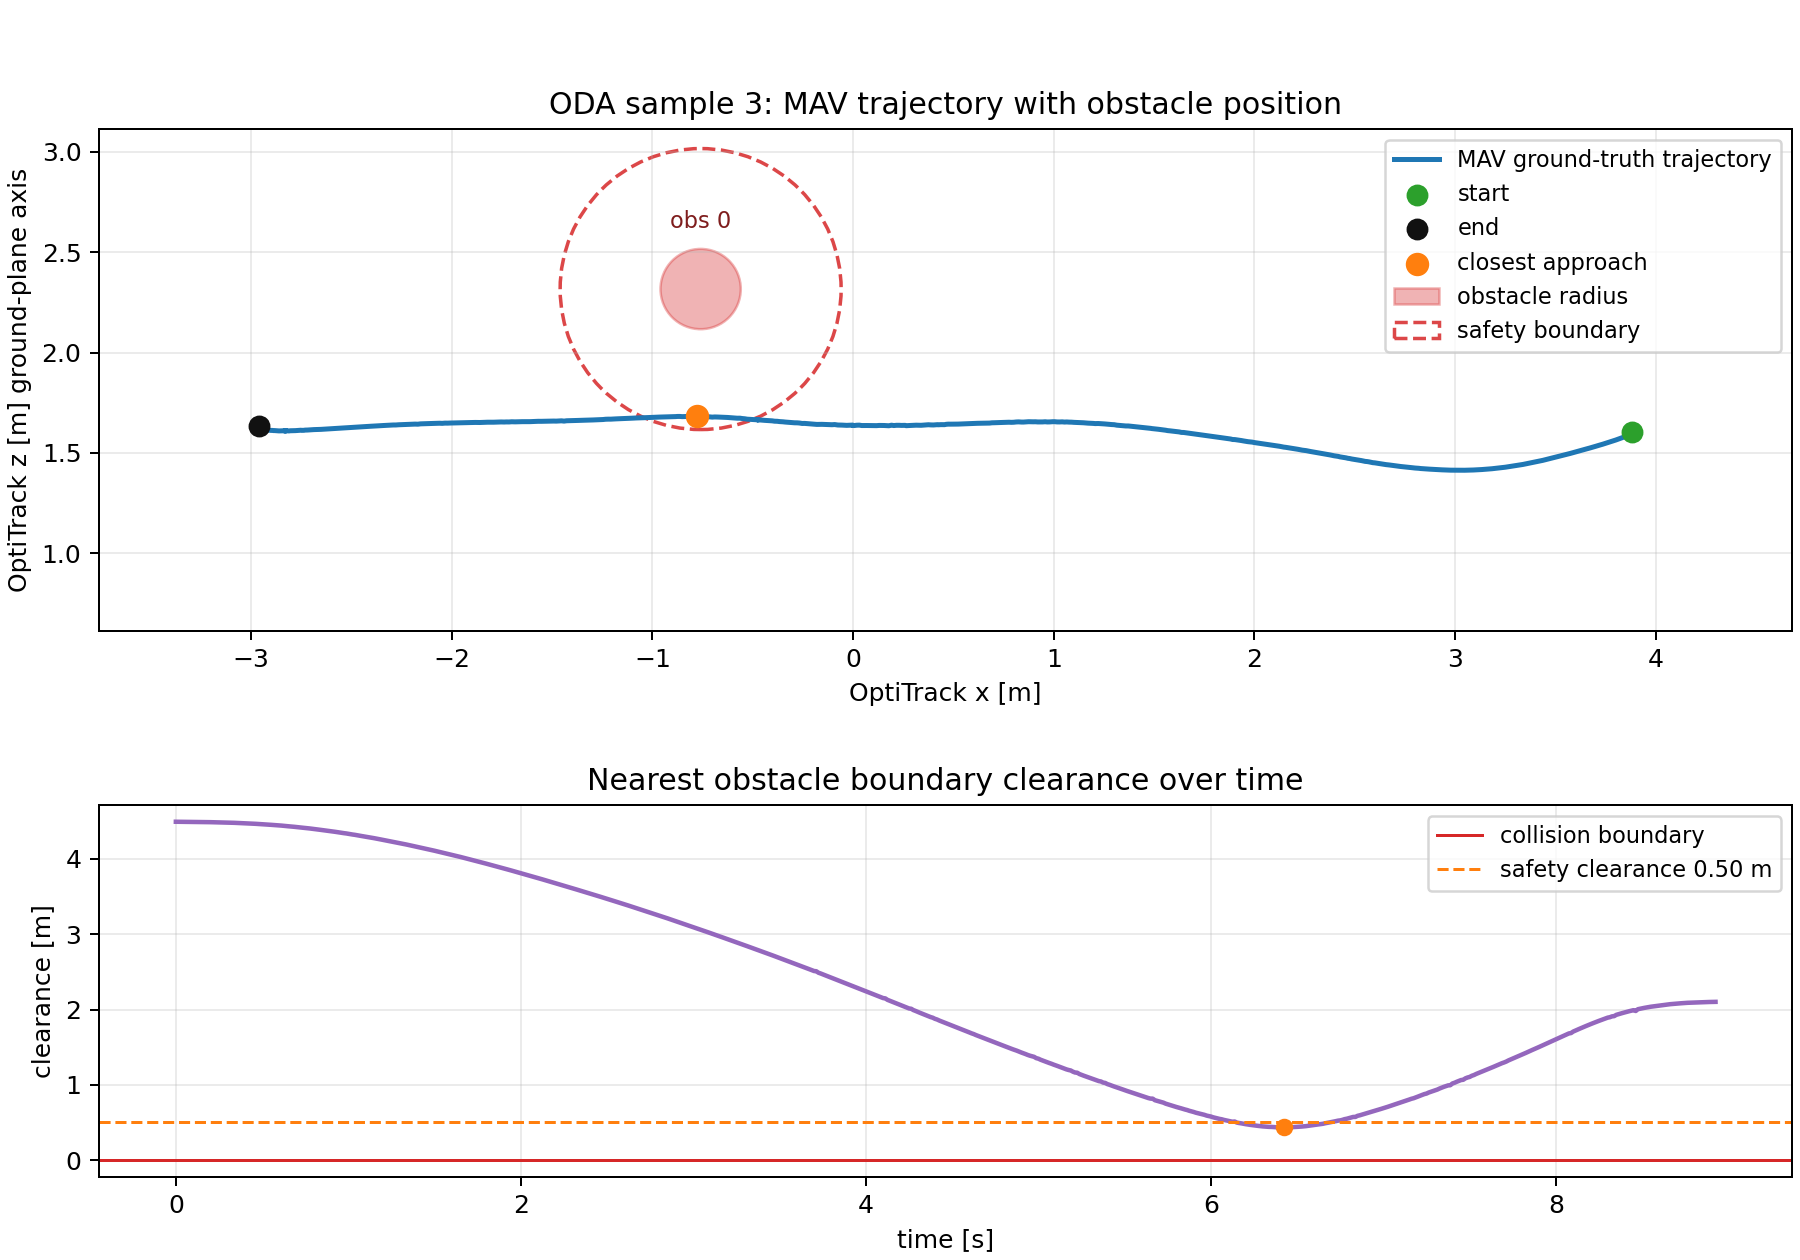
\includegraphics[width=\linewidth]{trajectory_sample_3.png}
\caption{Trial 3: vi phạm safety clearance.}
\end{subfigure}
\hfill
\begin{subfigure}{0.48\linewidth}
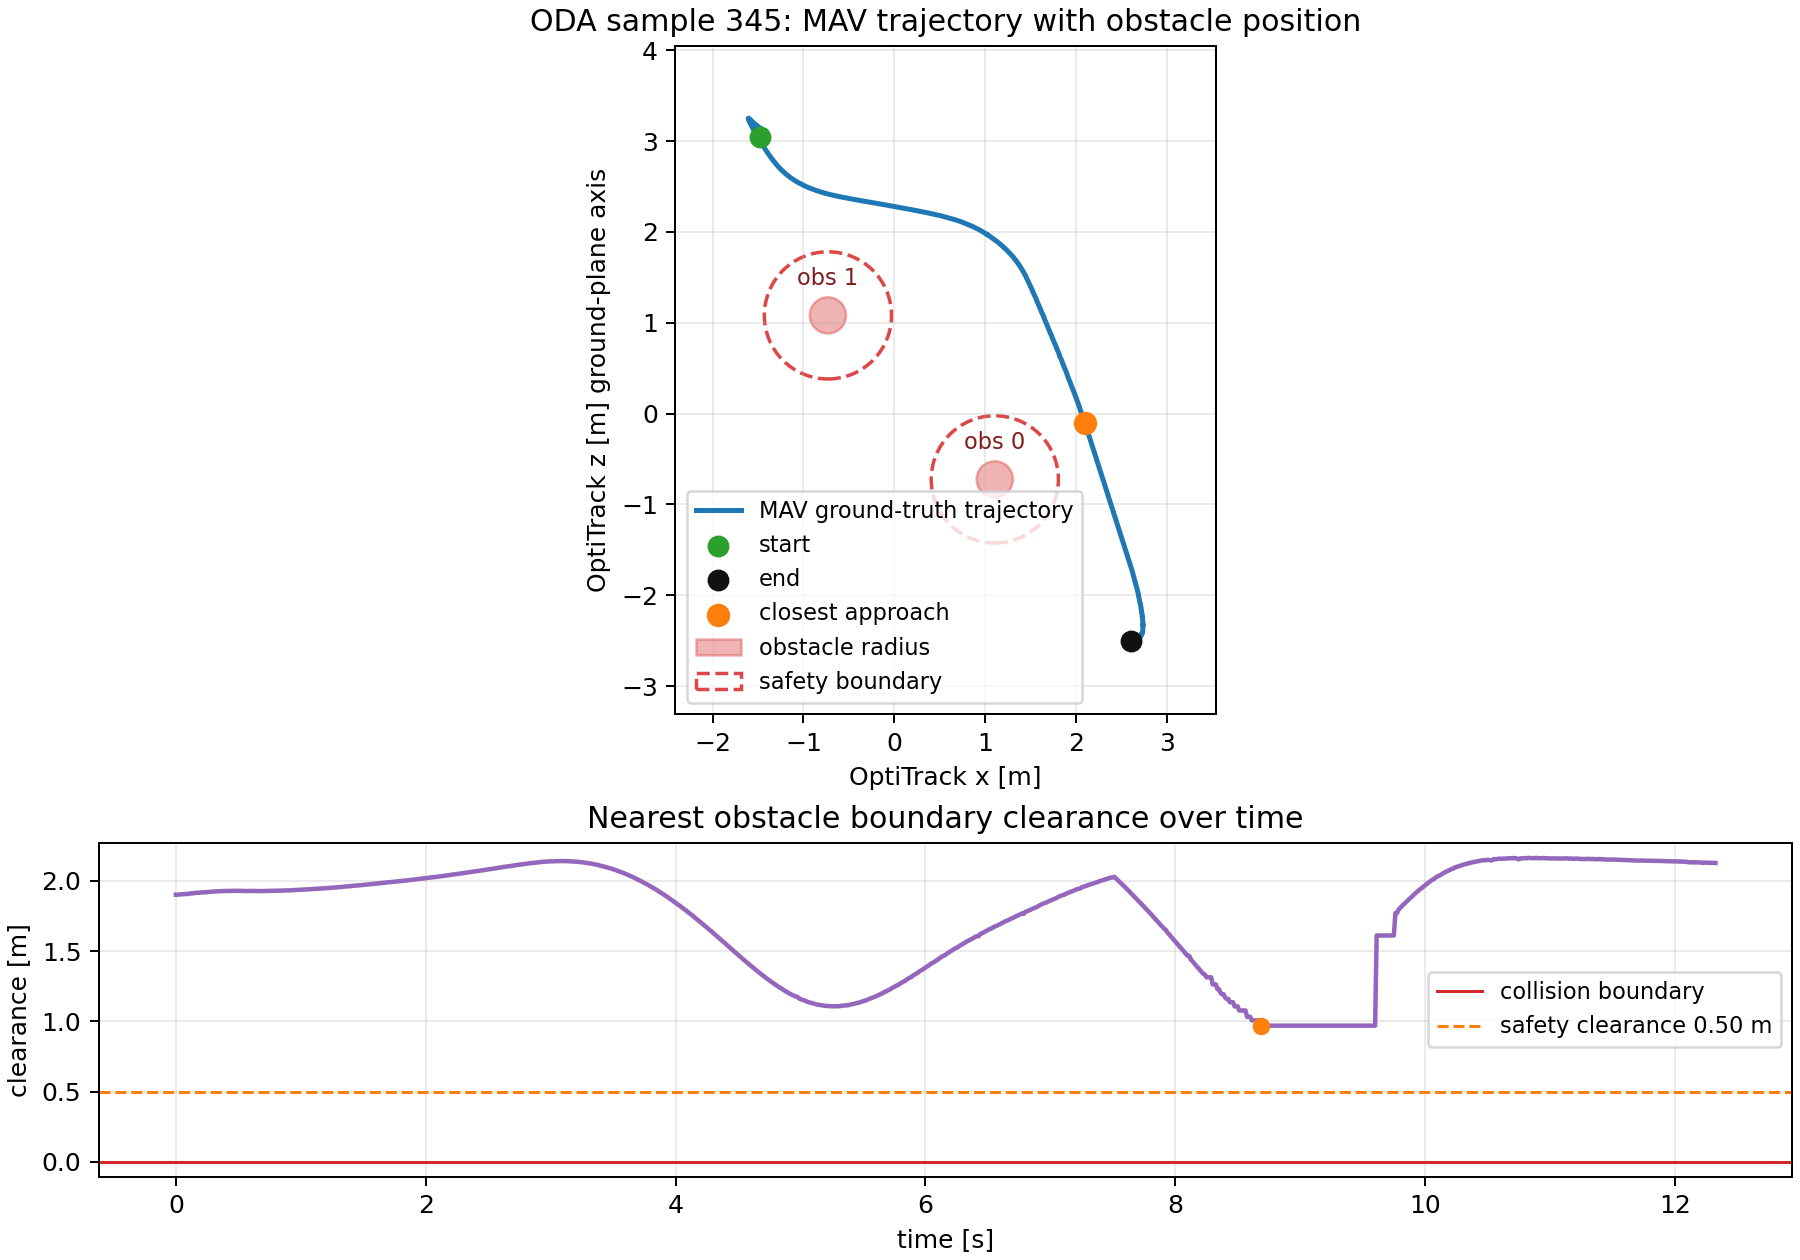
\includegraphics[width=\linewidth]{trajectory_sample_345.png}
\caption{Trial 345: hai vật cản, tránh an toàn.}
\end{subfigure}
\caption{Trajectory, obstacle boundary và clearance theo thời gian. Hai hình này là minh chứng trực tiếp rằng pipeline đọc được ground truth và biến nó thành metric an toàn.}
\end{figure}

\section{Biểu diễn vật cản}

Ở ODA, metadata cho vị trí vật cản trên mặt phẳng bay. Vì vậy biểu diễn chính là circle/cylinder 2D với bán kính vật cản và safety boundary. Để phù hợp yêu cầu bài toán, pipeline cũng xuất bounding box 2D và occupancy footprint. Với trial hai vật cản, diện tích bounding box trung bình lớn hơn nhiều vì phải bao phủ cả hai vùng vật cản.

\begin{table}[H]
\centering
\small
\caption{Obstacle representation trên 300 trial mục tiêu.}
\begin{tabular}{lrrrrrr}
\toprule
Obstacle count & Trials & Circle area & Inflated area & BBox area & Occupancy area & Fill ratio \\
\midrule
1 & 150 & 0.1257 & 1.5394 & 1.9600 & 1.5600 & 0.7959 \\
2 & 150 & 0.2513 & 3.0788 & 5.8380 & 3.0800 & 0.5476 \\
\bottomrule
\end{tabular}
\end{table}

\begin{figure}[H]
\centering
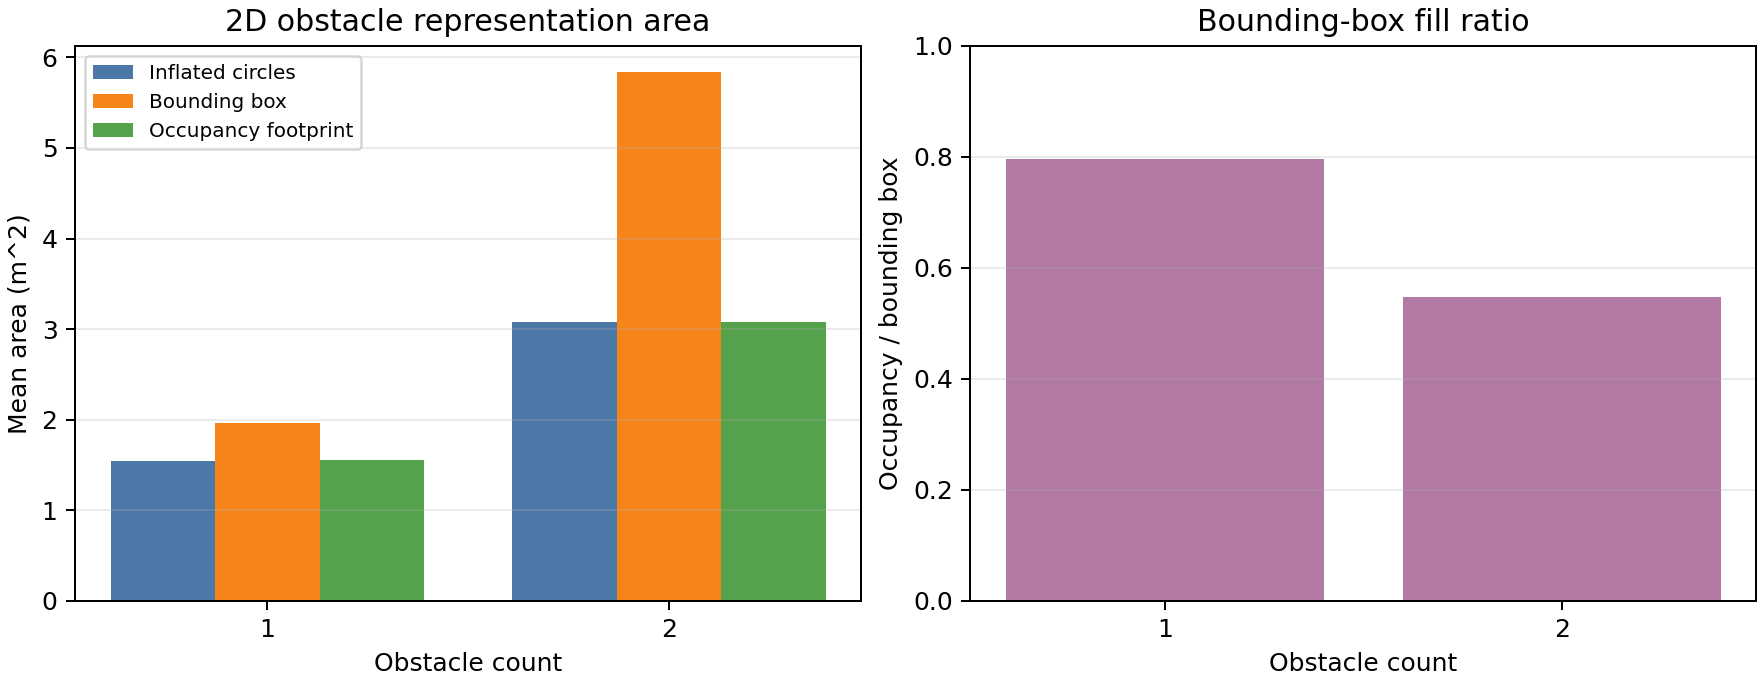
\includegraphics[width=0.72\linewidth]{obstacle_representation_summary.png}
\caption{Tóm tắt circle, inflated safety circle, bounding box và occupancy footprint. Đây là phần nối giữa yêu cầu ``biểu diễn vật cản'' và planner grid/sampling.}
\end{figure}

\section{Planner comparison trên 300 trial ODA}

Benchmark planner trả lời câu hỏi: nếu đã biết start, goal và vị trí vật cản từ ground truth, các phương pháp lập kế hoạch cổ điển có tạo được đường an toàn không? Đây là baseline quan trọng trước khi nói đến perception. Nếu planner còn không giải được bản đồ ground truth, thì thêm sensor/depth sẽ chưa có ý nghĩa. Kết quả hiện tại cho thấy planner hình học đã giải tốt phần này, nên hướng nâng tầm hợp lý là perception-risk và dynamic feasibility.

\begin{table}[H]
\centering
\small
\caption{So sánh planner trên 300 trial ODA.}
\begin{tabular}{lrrrrrr}
\toprule
Method & Trials & Coll. & Viol. & Clearance & Length & Time ms \\
\midrule
Human & 300 & 0.0733 & 0.4467 & 0.6126 & 6.6398 & 0.0000 \\
Straight-line & 300 & 0.1400 & 0.6533 & 0.4203 & 5.9686 & 2.8712 \\
Geometric bypass & 196 & 0.0000 & 0.0051 & 0.7005 & 6.3015 & 6.3860 \\
Geometric not-needed & 104 & 0.0000 & 0.0000 & 0.8647 & 5.6692 & 2.4630 \\
A* grid & 300 & 0.0000 & 0.0000 & 0.6426 & 6.2658 & 8.6793 \\
RRT & 300 & 0.0000 & 0.0000 & 0.6702 & 6.1940 & 3.6168 \\
RRT* & 300 & 0.0000 & 0.0000 & 0.6360 & 6.0122 & 1196.3979 \\
MPPI & 300 & 0.0000 & 0.0033 & 0.7574 & 6.0809 & 39.9327 \\
\bottomrule
\end{tabular}
\end{table}

\textbf{Cách diễn giải bảng này:}
\begin{itemize}
  \item Straight-line là baseline cố tình đơn giản. Nó ngắn nhưng unsafe: collision rate \(0.14\), violation rate \(0.6533\).
  \item Human trajectory không collision-free tuyệt đối trong metric hiện tại: collision rate \(0.0733\), violation rate \(0.4467\). Điều này không có nghĩa người lái kém; nó cho thấy threshold safety \(0.50\,m\) khá nghiêm và benchmark đang đo rủi ro gần vật cản.
  \item A*, RRT và RRT* đạt \(0.00\) collision/violation trên 300 trial. Đây là bằng chứng obstacle-aware planner tạo được đường an toàn khi biết bản đồ.
  \item MPPI có mean clearance cao nhất \(0.7574\,m\), nhưng vẫn có violation nhỏ \(0.0033\) và compute time cao hơn A*/RRT trong prototype Python.
  \item RRT* chậm nhất vì có rewiring/neighborhood optimization; đây là trade-off kinh điển giữa chất lượng đường đi và thời gian tính.
\end{itemize}

\begin{figure}[H]
\centering
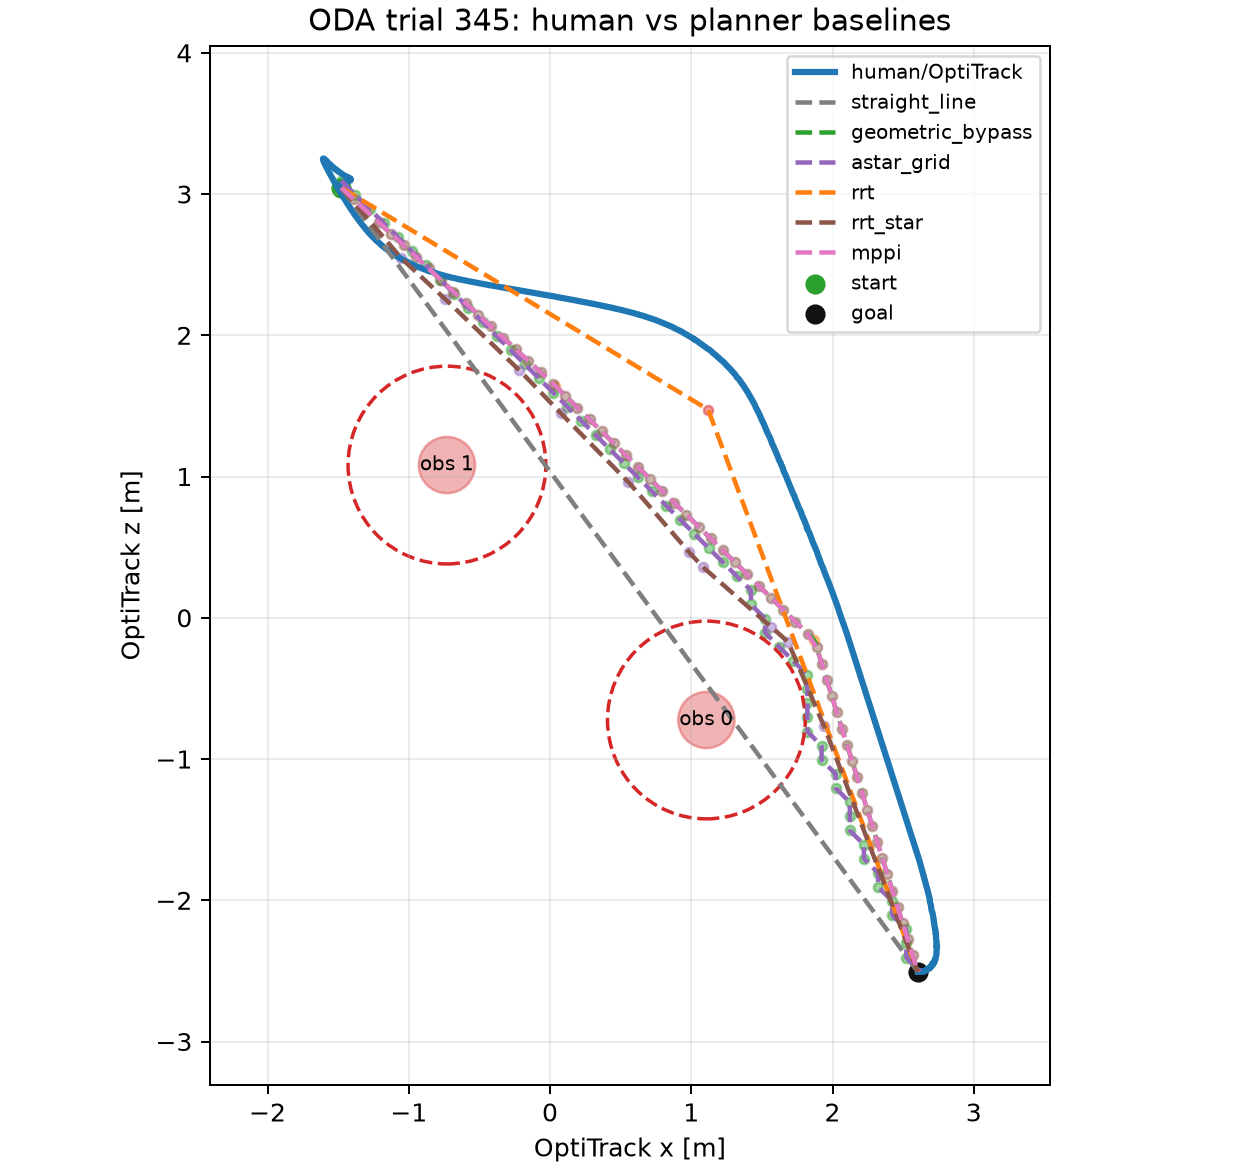
\includegraphics[width=0.84\linewidth]{planner_comparison_sample_345.png}
\caption{Planner comparison trên trial 345. Hình này nên dùng khi giải thích trực quan: straight-line có thể đi qua vùng nguy hiểm, còn planner obstacle-aware tạo đường vòng an toàn.}
\end{figure}

\section{Sampling-based planning và optimization-based methods}

Để trả lời đúng yêu cầu bài toán, cần phân loại rõ các phương pháp.

\begin{table}[H]
\centering
\small
\caption{Phân loại phương pháp trong project.}
\begin{tabularx}{0.96\linewidth}{>{\bfseries}p{3.2cm} p{3.2cm} X}
\toprule
Nhóm & Phương pháp & Vai trò trong project \\
\midrule
Search-based planning & A* grid & Rời rạc hóa mặt phẳng bay thành occupancy grid, sau đó tìm đường có chi phí thấp bằng heuristic. Đây là baseline cổ điển, dễ giải thích và chạy nhanh. \\
Sampling-based planning & RRT, RRT* & Lấy mẫu trong không gian 2D, nối mẫu nếu collision-free. RRT nhanh; RRT* thêm rewiring để tiến tới tối ưu hơn nhưng chậm. \\
Optimization-based / sampling-based optimal control & MPPI & Sinh nhiều rollout/trajectory ứng viên, chấm điểm bằng cost gồm goal, clearance penalty, path length, smoothness và collision penalty. Đây là cầu nối gần MPC hơn, nhưng bản hiện tại vẫn là Python 2D nhẹ. \\
Geometric baseline & Straight-line, geometric bypass & Dùng để tạo mốc so sánh dễ hiểu: đường thẳng unsafe, bypass đơn giản nhưng hiệu quả trong nhiều case. \\
\bottomrule
\end{tabularx}
\end{table}

Trong báo cáo nên nói cẩn thận: MPPI là optimization-based theo nghĩa tối ưu chi phí trên rollout, đồng thời cũng là sampling-based optimal control. Nó chưa phải MPC đầy đủ với dynamic model/constraint của quadrotor, nên không nên claim ``đã triển khai MPC UAV hoàn chỉnh''.

\section{Trajectory smoothness và dynamic feasibility proxy}

Tránh vật cản không chỉ là không va chạm. Một quỹ đạo bay thực tế cần đủ mượt, không đổi hướng quá gắt và không vượt giới hạn động học. Trong giai đoạn này, pipeline đo proxy 2D: path length, mean speed và heading-change smoothness. Đây là một bước đúng để trả lời yêu cầu ``tính khả thi động học'', nhưng vẫn cần nói rõ chưa phải kiểm chứng full dynamics của quadrotor.

\begin{table}[H]
\centering
\small
\caption{Proxy feasibility trên 300 trial.}
\begin{tabular}{lrrrrr}
\toprule
Method & Mean speed & P95 speed & Smoothness & P95 smooth. & Time ms \\
\midrule
Human & 0.7371 & 1.2639 & 0.679198 & 1.404319 & 0.0000 \\
A* grid & 0.7064 & 1.2933 & 0.005906 & 0.014213 & 8.6793 \\
RRT & 0.6976 & 1.2481 & 0.000551 & 0.002657 & 3.6168 \\
RRT* & 0.6766 & 1.2360 & 0.000062 & 0.000279 & 1196.3979 \\
MPPI & 0.6841 & 1.2460 & 0.000104 & 0.000418 & 39.9327 \\
\bottomrule
\end{tabular}
\end{table}

\begin{figure}[H]
\centering
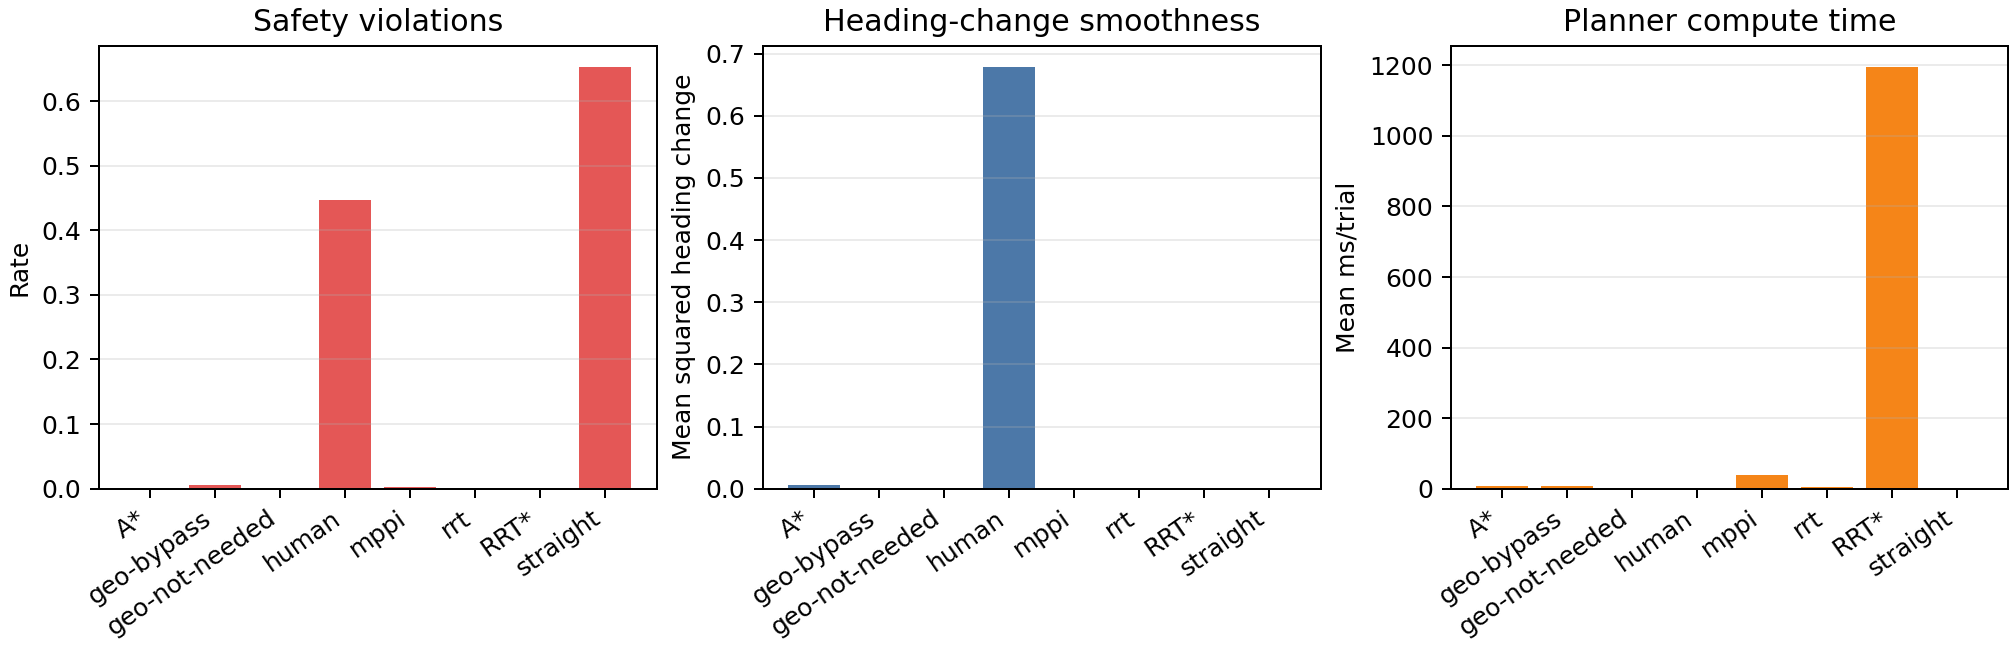
\includegraphics[width=0.76\linewidth]{trajectory_feasibility_summary.png}
\caption{Trajectory feasibility proxy. Khi bảo vệ, nên nói rõ đây là proxy từ 2D path/speed/heading-change, chưa phải jerk/snap/actuator constraint.}
\end{figure}

\section{Perception-risk: depth, radar và IMU}

Sau khi planner benchmark ổn định, câu hỏi nghiên cứu chuyển từ ``có đường tránh không?'' sang ``sensor có cảnh báo được nguy cơ không?''. Pipeline dùng ba nhóm feature:
\begin{itemize}
  \item \textbf{Depth:} \code{depth\_min}, \code{depth\_p10}, \code{depth\_median} trong center crop của predicted depth.
  \item \textbf{Radar:} peak, peak range-bin, energy và range-Doppler summary.
  \item \textbf{IMU:} norm của acceleration và gyroscope, phản ánh trạng thái chuyển động/điều khiển.
\end{itemize}

Bảng Depth Anything V2 Small trên 50 trial có 2584 frame. Phân bố nhãn bị lệch mạnh: 2294 safe, 171 warning, 119 danger; future-risk có 241 frame dương và 2343 frame âm. Vì vậy metric chính phải là macro-F1, balanced accuracy và recall future-risk, không chỉ accuracy.

\begin{table}[H]
\centering
\small
\caption{Perception-risk với Depth Anything V2 Small trên 50 trial.}
\begin{tabular}{lrrrrr}
\toprule
Feature group & Threshold & Accuracy & Macro-F1 & Bal. acc. & Risk recall \\
\midrule
Radar, macro-F1 tuned & 0.80 & 0.9053 & 0.4894 & 0.5072 & 0.0145 \\
Depth, macro-F1 tuned & 0.90 & 0.8872 & 0.4821 & 0.4972 & 0.0145 \\
Radar+IMU, macro-F1 tuned & 0.80 & 0.9025 & 0.4744 & 0.4992 & 0.0000 \\
Depth+radar+IMU, macro-F1 tuned & 0.40 & 0.9011 & 0.5918 & 0.5697 & 0.1594 \\
Radar, recall tuned & 0.05 & 0.4889 & 0.3995 & 0.5100 & 0.5362 \\
Depth, recall tuned & 0.05 & 0.7382 & 0.5504 & 0.6220 & 0.4783 \\
Radar+IMU, recall tuned & 0.05 & 0.4930 & 0.4165 & 0.5771 & 0.6812 \\
Depth+radar+IMU, recall tuned & 0.05 & 0.6602 & 0.5260 & 0.6631 & 0.6667 \\
\bottomrule
\end{tabular}
\end{table}

Kết luận quan trọng ở đây là trade-off. Nếu tối ưu macro-F1/accuracy, mô hình ít báo nguy hiểm hơn nhưng ổn định hơn. Nếu ưu tiên recall future-risk, mô hình báo động nhiều hơn và accuracy giảm, nhưng bỏ sót nguy cơ ít hơn. Với hệ safety-critical, cấu hình recall-tuned có thể đáng quan tâm hơn, miễn là sau này có cơ chế giảm false alarm.

\begin{figure}[H]
\centering
\begin{subfigure}{0.48\linewidth}
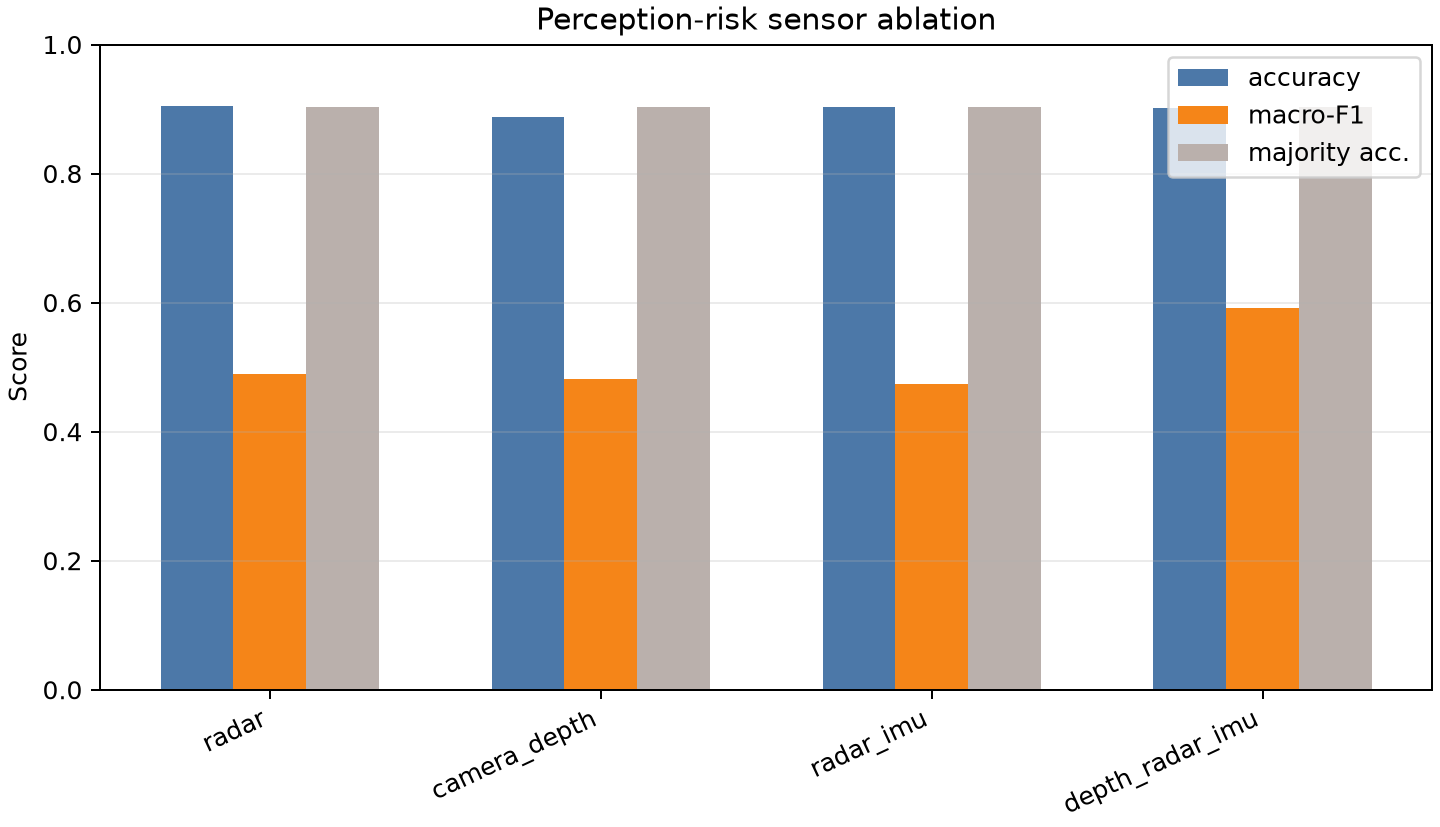
\includegraphics[width=\linewidth]{perception_risk_ablation_balanced_depth_anything_v2_small_50.png}
\caption{Macro-F1 tuned.}
\end{subfigure}
\hfill
\begin{subfigure}{0.48\linewidth}
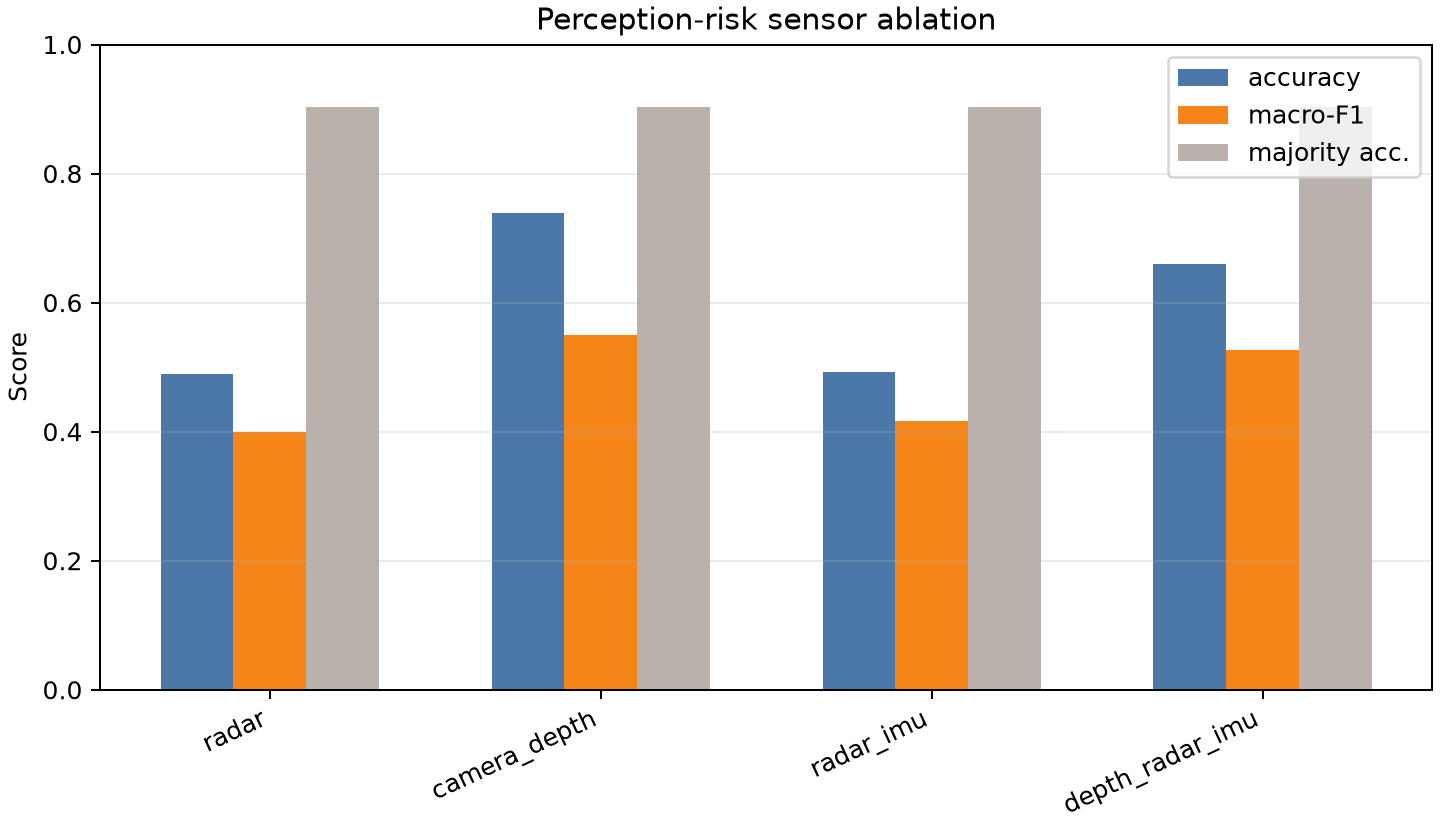
\includegraphics[width=\linewidth]{perception_risk_ablation_recall_tuned_depth_anything_v2_small_50.png}
\caption{Recall tuned.}
\end{subfigure}
\caption{Ablation perception-risk. Hình này giúp kể câu chuyện mất cân bằng nhãn và trade-off giữa accuracy và risk recall.}
\end{figure}

\section{Monocular depth: kết quả, tốc độ và giới hạn}

Depth panel hiện dùng monocular predicted depth từ RGB frame. Đây là relative depth, không phải metric depth theo mét. Điểm này cần nói rõ vì nếu mentor hỏi ``độ sâu có đúng mét không?'', câu trả lời phải là: hiện tại chưa, em dùng như cue tương đối và feature rủi ro; bước tiếp theo là hiệu chuẩn với OptiTrack clearance/radar.

\begin{table}[H]
\centering
\small
\caption{Timing depth inference.}
\begin{tabular}{lrrrr}
\toprule
Model/backend & Trials & Frames & Wall s/frame & Infer s/frame \\
\midrule
DPT-Hybrid/MiDaS, PyTorch & 20 & 1096 & 0.088463 & 0.042238 \\
DPT-Hybrid/MiDaS, ONNX CUDA probe & 3 & 177 & 0.082662 & 0.040498 \\
Depth Anything V2 Small, PyTorch batch & 50 & 2584 & 0.063874 & 0.017378 \\
\bottomrule
\end{tabular}
\end{table}

Depth Anything V2 Small nhanh hơn DPT trong batch run hiện tại, đặc biệt ở inference-time. Tuy nhiên tốc độ wall-time vẫn bị ảnh hưởng bởi decode video, preprocessing, resize và ghi cache \code{npz}. Đây là lý do không nên chỉ nhìn kích thước model để kết luận tốc độ thực tế.

\begin{table}[H]
\centering
\small
\caption{Depth stability/calibration hiện tại.}
\begin{tabular}{lrrrr}
\toprule
Model & Rows & Spearman depth-clearance & Linear RMSE m & Mean abs depth delta \\
\midrule
DPT-Hybrid/MiDaS & 1096 & 0.4752 & 1.1950 & 4.7859 \\
Depth Anything V2 Small 50 & 2584 & 0.3251 & 1.1733 & 5.2004 \\
\bottomrule
\end{tabular}
\end{table}

\begin{figure}[H]
\centering
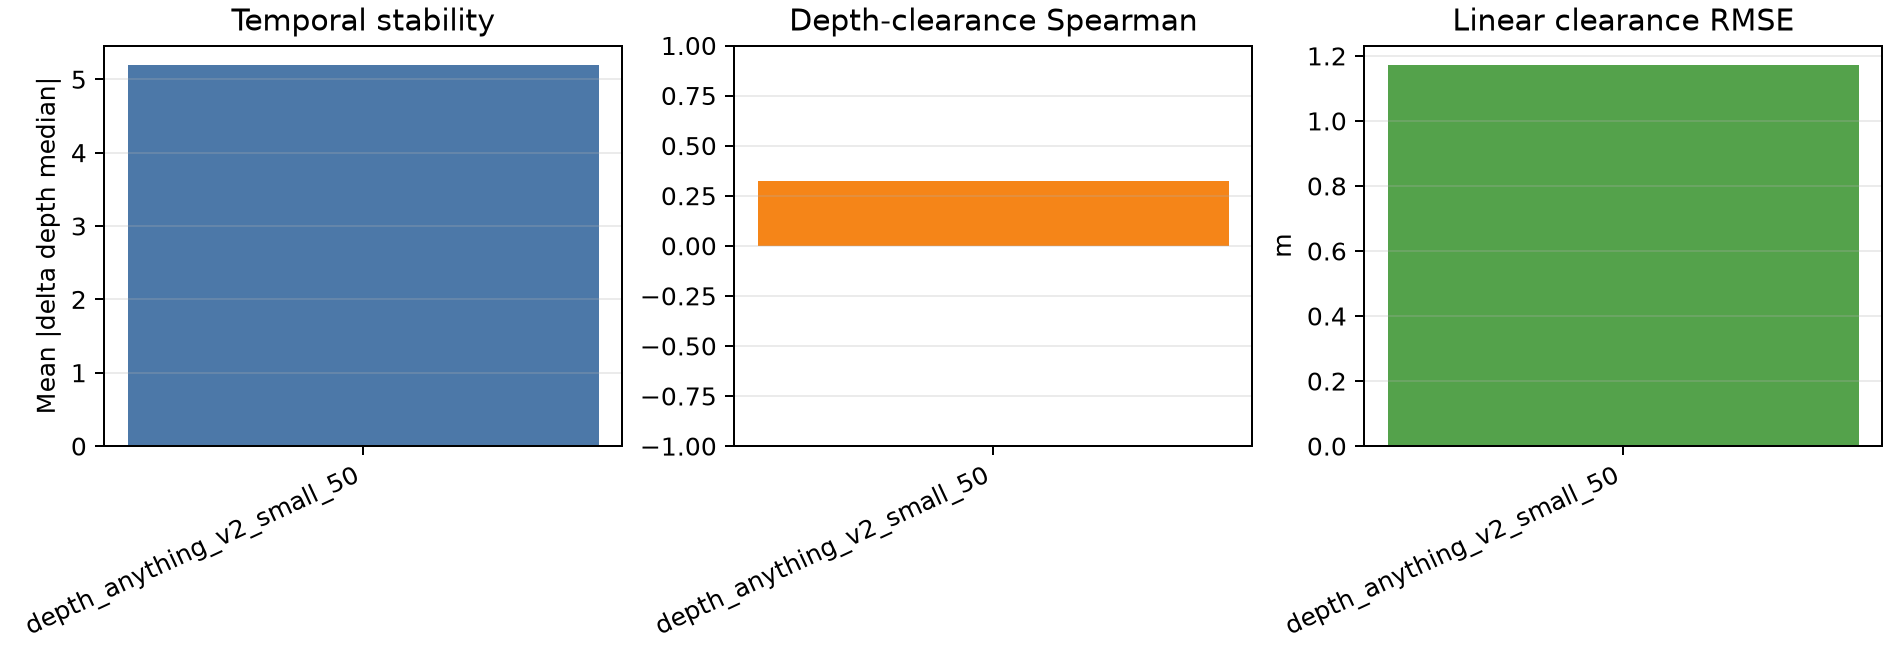
\includegraphics[width=0.78\linewidth]{depth_stability_calibration_depth_anything_v2_small_50.png}
\caption{Phân tích stability/calibration cho Depth Anything V2 Small. Kết quả đủ để dùng depth như cue tương đối, chưa đủ để claim metric depth.}
\end{figure}

\section{Radar range-Doppler và IMU}

ODA có radar 24 GHz. Pipeline hiện đã đọc radar CSV, tạo FFT/peak/energy cho video panel và bổ sung phân tích range-Doppler. Range-Doppler giúp tách hai câu hỏi: vật thể/đáp ứng mạnh nằm ở range bin nào, và có tín hiệu Doppler tương đối như thế nào. Đây là phần làm report có tính đa cảm biến thật hơn, thay vì chỉ camera-based.

\begin{table}[H]
\centering
\small
\caption{Radar range-Doppler summary trên ba sample.}
\begin{tabular}{lrrrrrr}
\toprule
Trial & Sweeps & Range bins & Mean range bin & Mode range bin & Zero-Doppler frac. & Mean entropy \\
\midrule
3 & 139 & 128 & 21.7842 & 15 & 0.1727 & 8.9222 \\
10 & 225 & 128 & 16.9644 & 3 & 0.5689 & 8.4488 \\
345 & 192 & 128 & 13.7188 & 6 & 0.5260 & 8.5293 \\
\bottomrule
\end{tabular}
\end{table}

\begin{figure}[H]
\centering
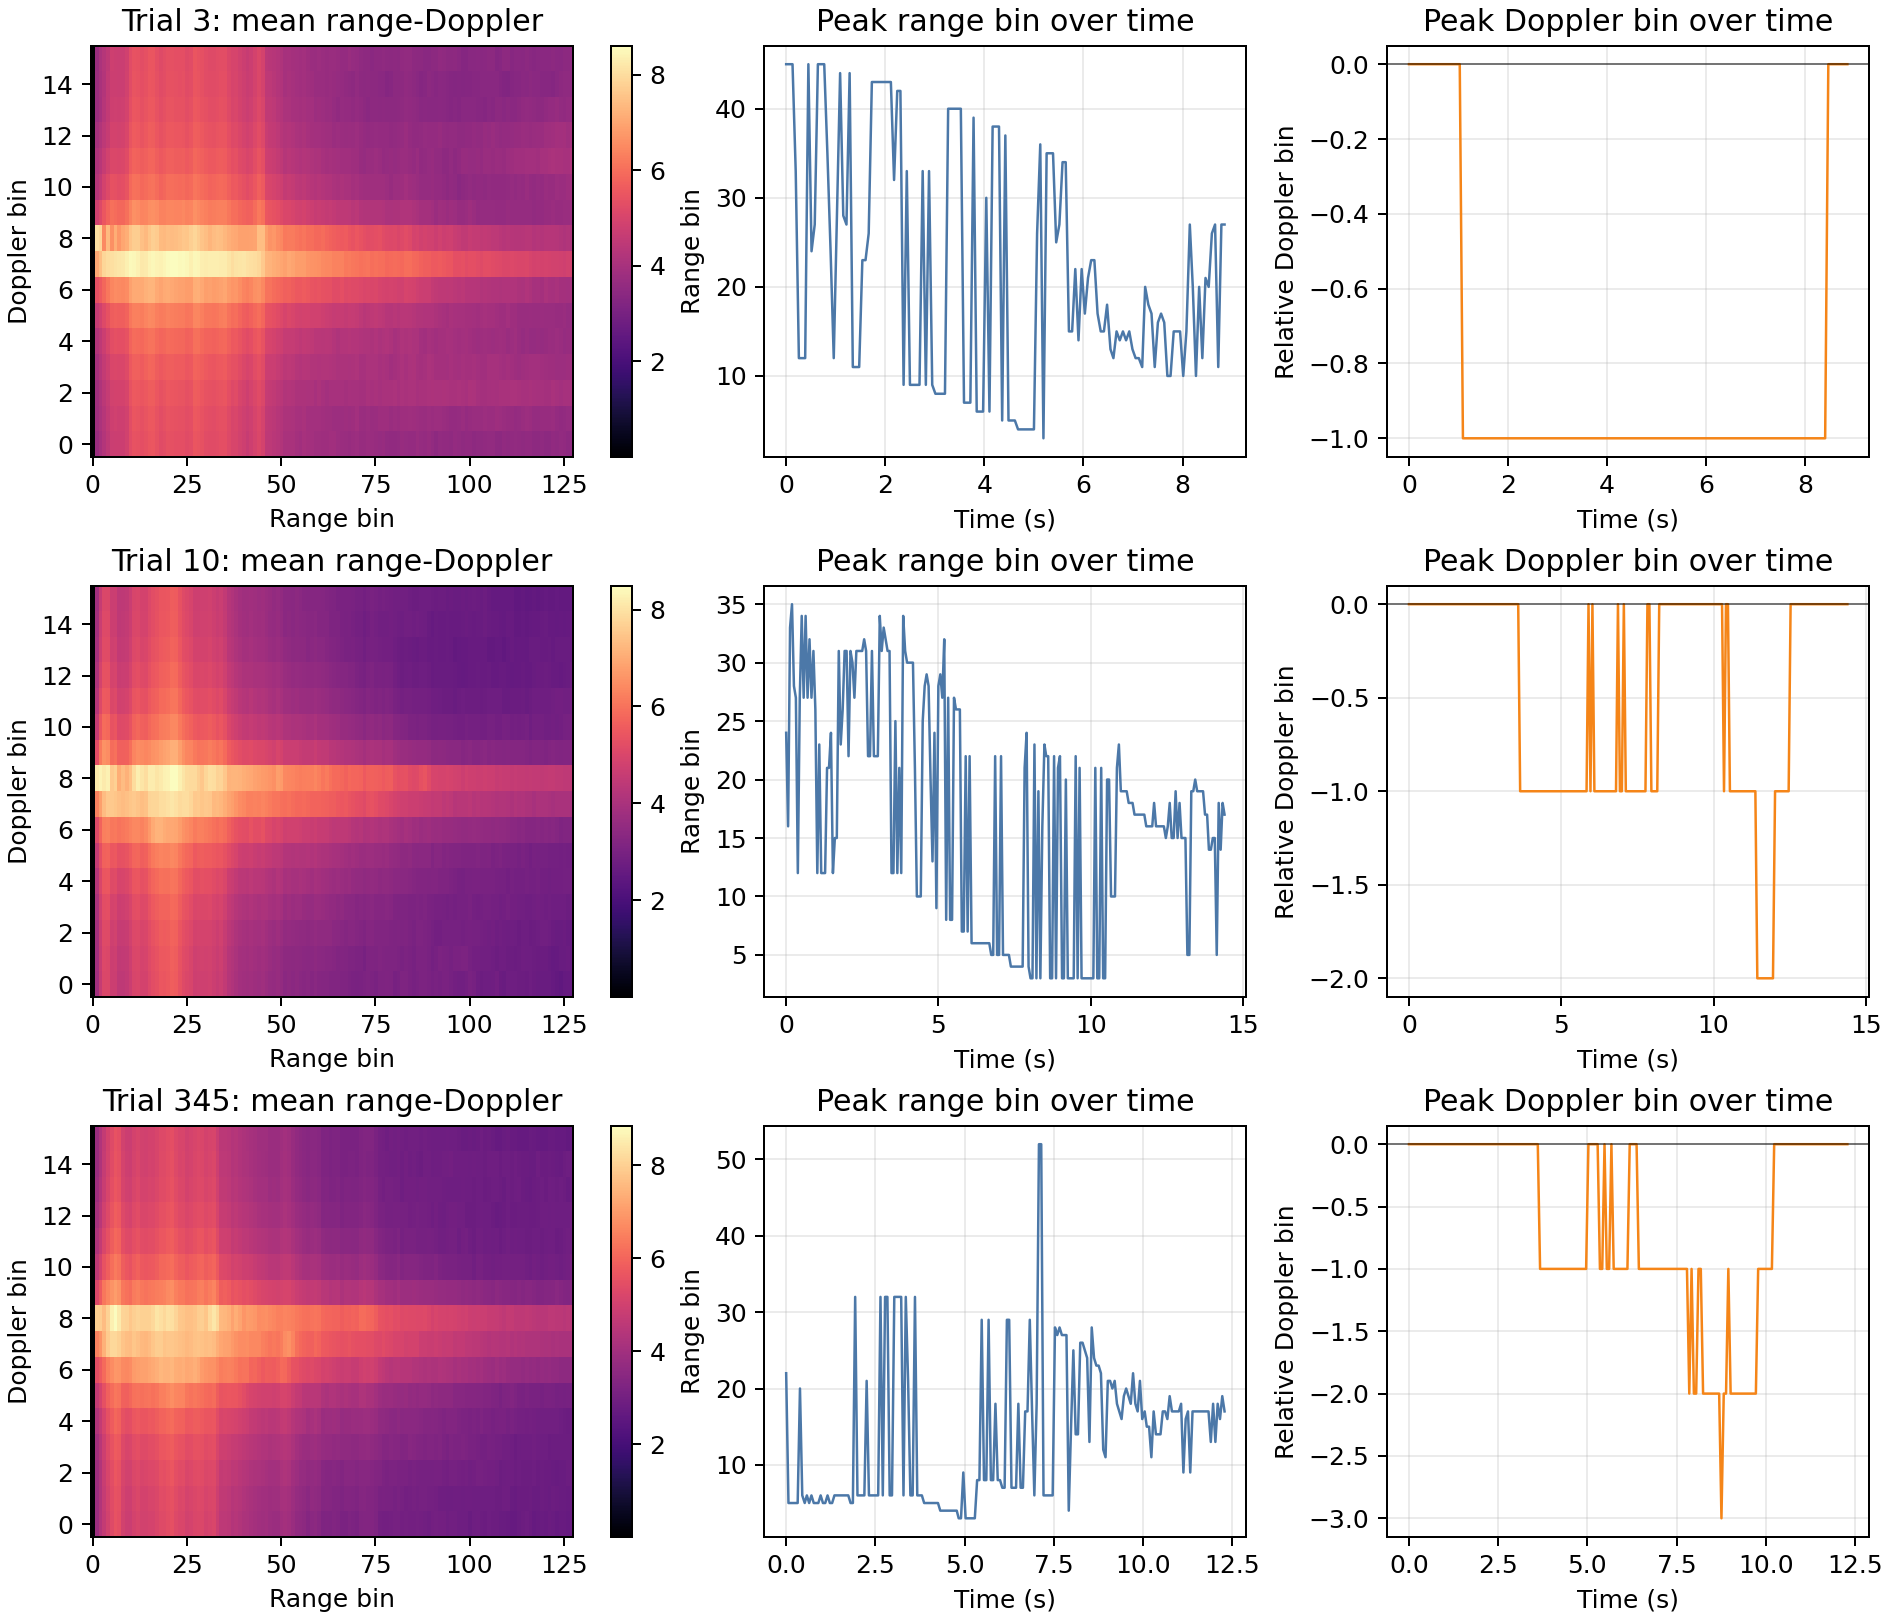
\includegraphics[width=0.82\linewidth]{radar_range_doppler_summary.png}
\caption{Range-Doppler summary. Trong câu chuyện nghiên cứu, radar là cảm biến bổ sung giúp kiểm tra risk cue không chỉ dựa vào RGB/depth.}
\end{figure}

IMU không phải obstacle detector, nhưng nó cung cấp bối cảnh chuyển động: UAV đang ổn định, tăng tốc hay đổi hướng mạnh. Trong video 5/6 panel, IMU rolling plot giúp mentor thấy pipeline đang đồng bộ nhiều luồng dữ liệu theo thời gian.

\section{LiDAR point cloud segmentation, clustering và 3D bounding box}

Ban đầu ODA là benchmark chính, nhưng yêu cầu bài toán có nhắc LiDAR/point cloud. ODA không phải LiDAR benchmark chính, vì vậy cách xử lý hợp lý là dùng external dataset như ARCO và Multi-LiDAR để chứng minh pipeline có nhánh point cloud thật. Nhánh này không thay đổi kết quả planner ODA; nó bổ sung năng lực perception.

Script point cloud hiện không cần ROS runtime. Nó đọc bag bằng \code{rosbags}, decode \code{sensor\_msgs/PointCloud2} hoặc Livox \code{CustomMsg}, lọc vùng quan tâm, loại ground bằng percentile, voxel hóa, gom connected components, sau đó xuất 3D axis-aligned bounding boxes.

\begin{table}[H]
\centering
\small
\caption{Kết quả point-cloud processing thật trên ARCO và Multi-LiDAR.}
\begin{tabular}{lrrrrr}
\toprule
Nguồn & Frames & Raw pts/frame & FG pts/frame & Clusters/frame & 3D boxes \\
\midrule
ARCO Ouster & 6 & 26324 & 9401 & 4.17 & 25 \\
Calibration Ouster & 8 & 57525 & 21403 & 3.50 & 28 \\
Calibration depth cloud & 8 & 117636 & 10422 & 1.00 & 8 \\
HolybroStdn01 Ouster & 8 & 57817 & 17594 & 8.62 & 69 \\
HolybroStdn01 Mid360 & 8 & 2004 & 1212 & 5.00 & 40 \\
HolybroStdn01 Avia & 8 & 2400 & 809 & 6.38 & 51 \\
TelloOut02 Ouster & 8 & 43209 & 6385 & 3.25 & 26 \\
TelloOut02 Mid360 & 8 & 1992 & 503 & 1.12 & 9 \\
TelloOut02 Avia & 8 & 2400 & 1748 & 1.62 & 13 \\
Tello03 Ouster & 8 & 58044 & 17530 & 7.62 & 61 \\
Tello03 Mid360 & 8 & 2004 & 1173 & 5.38 & 43 \\
Tello03 Avia & 8 & 2400 & 1042 & 5.62 & 45 \\
\bottomrule
\end{tabular}
\end{table}

Kết quả mới nhất là hai bag Tello03 và TelloOut02. Hai bag này có cùng cấu trúc sensor với HolybroStdn01: Ouster PointCloud2, Livox Mid360 CustomMsg, Livox Avia CustomMsg, camera RGB, IMU và pose OptiTrack/VRPN. Tello03 tạo nhiều cụm hơn TelloOut02: tổng 149 bbox 3D trên 24 sensor-frame, so với 48 bbox trên TelloOut02. Điều này hữu ích cho câu chuyện tiến độ vì nó cho thấy pipeline không chỉ chạy được trên một file may mắn, mà đã bắt đầu kiểm tra độ ổn định qua nhiều bag Multi-LiDAR.

\begin{figure}[H]
\centering
\includegraphics[width=0.96\linewidth]{multilidar_tello03_ouster_pointcloud_3d_bboxes.png}
\caption{Multi-LiDAR Tello03 Ouster: segmentation/clustering/3D bbox thật. Hình được để lớn để thấy rõ cụm point cloud và các hộp 3D, thay vì chỉ dùng như minh họa nhỏ.}
\end{figure}

\begin{figure}[H]
\centering
\begin{subfigure}{0.48\linewidth}
\includegraphics[width=\linewidth]{multilidar_tello03_mid360_livox_3d_bboxes.png}
\caption{Tello03 Mid360.}
\end{subfigure}
\hfill
\begin{subfigure}{0.48\linewidth}
\includegraphics[width=\linewidth]{multilidar_tello03_avia_livox_3d_bboxes.png}
\caption{Tello03 Avia.}
\end{subfigure}
\caption{Tello03 trên hai sensor Livox. Hai hình này bổ sung cho Ouster để chứng minh pipeline xử lý được cả \code{PointCloud2} và Livox \code{CustomMsg}.}
\end{figure}

\begin{figure}[H]
\centering
\includegraphics[width=0.96\linewidth]{multilidar_telloout02_ouster_pointcloud_3d_bboxes.png}
\caption{Multi-LiDAR TelloOut02 Ouster: cùng pipeline nhưng trong scene khác. Số cụm ít hơn Tello03, giúp minh họa độ biến thiên theo môi trường/sensor sequence.}
\end{figure}

Khi trình bày, nên nói: ARCO là ground-robot dataset nên không so sánh trực tiếp với ODA; Multi-LiDAR là UAV/multi-sensor stress-test nhưng chưa dùng để đánh giá obstacle avoidance trajectory. Việc tách rạch ròi như vậy giúp project không bị loãng.

\section{Kết quả định tính nên trình bày}

Khi gặp mentor, nên mở một video trước khi nói bảng số liệu. Video giúp người nghe hiểu ngay project đang làm gì. Sau đó mới chuyển sang metric.

\begin{table}[H]
\centering
\small
\caption{Các video nên dùng trong buổi trao đổi.}
\begin{tabularx}{0.96\linewidth}{>{\bfseries}p{4.4cm} X}
\toprule
Video & Nên nói gì khi mở video \\
\midrule
\begin{tabular}{@{}l@{}}\code{qualitative\_depth\_sensor}\\\code{\_sample\_3.mp4}\end{tabular} & Đây là case safety-distance violation. Em hiển thị RGB, relative depth, radar FFT, IMU, safety map và trajectory cùng lúc để thấy rủi ro theo thời gian. \\
\begin{tabular}{@{}l@{}}\code{qualitative\_depth\_sensor}\\\code{\_sample\_345.mp4}\end{tabular} & Đây là case hai vật cản, MAV tránh an toàn hơn. Dùng để cho thấy pipeline xử lý được nhiều vật cản. \\
\begin{tabular}{@{}l@{}}\code{qualitative\_sensor}\\\code{\_sample\_3.mp4}\end{tabular} & Nếu muốn tránh tranh luận về depth, mở bản 5 panel chỉ gồm sensor thật của ODA: RGB, radar, IMU, safety map, trajectory. \\
\bottomrule
\end{tabularx}
\end{table}

\begin{figure}[H]
\centering
\includegraphics[width=0.98\linewidth]{qualitative_depth_sensor_sample_345_contact_sheet_vertical.png}
\caption{Contact sheet dọc của video 6 panel cho trial 345. Trial này dùng tốt để kể câu chuyện hai vật cản và avoidance an toàn; bố cục dọc giúp từng panel đọc được khi in PDF.}
\end{figure}

\section{Đánh giá theo tiêu chí chấm điểm}

\begin{longtable}{>{\bfseries}p{3.2cm} p{11.4cm}}
\caption{Đối chiếu với tiêu chí hội đồng.}\\
\toprule
Tiêu chí & Nội dung có thể trình bày \\
\midrule
\endfirsthead
\toprule
Tiêu chí & Nội dung có thể trình bày \\
\midrule
\endhead
Độ khó, độ phức tạp & Bài toán kết hợp UAV indoor/GNSS-denied, dữ liệu đa cảm biến, trajectory ground truth, risk metric, planner comparison, predicted depth và point-cloud processing. Độ khó không nằm ở một model đơn lẻ mà ở việc nối được dữ liệu, metric, planner và perception thành một pipeline tái lập. \\
Quy mô công việc & Đã mở rộng từ 3 sample ban đầu lên 300 ODA trial cho planner, 50 trial cho depth/risk feature, nhiều video định tính, và nhiều nhánh external sensing trên ARCO/Multi-LiDAR. Có mã nguồn, bảng CSV, hình PNG, video MP4 và report. \\
Tính độc đáo/sáng tạo & Biến ODA từ dataset quan sát thành benchmark risk-aware: safety map, future-risk label, planner comparison, radar range-Doppler, IMU rolling feature, monocular depth cue, imbalance-aware classifier và LiDAR 3D bbox. \\
Mức độ hoàn thiện & Có pipeline chạy được end-to-end cho ODA; có benchmark 300 trial; có qualitative video; có depth timing; có risk classifier baseline; có LiDAR point-cloud segmentation thật. Các giới hạn được nêu rõ thay vì claim quá mức. \\
Phần bảo vệ & Có thể trả lời về vì sao dùng ODA, vì sao chưa dùng ROS/Gazebo, đâu là sampling-based/optimization-based method, depth có phải metric không, LiDAR được dùng thế nào, smoothness hiện đo ra sao và bước tiếp theo là gì. \\
\bottomrule
\end{longtable}

\section{Giới hạn hiện tại}

Một report tốt không chỉ nêu thành công. Nó cần biết phần nào chưa nên claim.

\begin{itemize}
  \item \textbf{Depth chưa phải metric depth:} Depth Anything/DPT hiện là relative depth. Cần calibration với OptiTrack clearance/radar trước khi dùng như khoảng cách theo mét.
  \item \textbf{TensorRT chưa có engine thật:} ONNX Runtime CUDA đã chạy, nhưng TensorRT provider thiếu runtime \code{libnvinfer.so.10}/\code{trtexec}, nên chưa claim speedup TensorRT.
  \item \textbf{Dynamic feasibility còn là proxy:} Smoothness/speed/path length mới là proxy 2D. Quadrotor thật cần ràng buộc velocity, acceleration, jerk/snap và actuator limit.
  \item \textbf{External datasets không trực tiếp so sánh với ODA:} ARCO là ground robot; Multi-LiDAR dùng cho stress-test point cloud. ODA vẫn là benchmark UAV obstacle avoidance chính.
  \item \textbf{Risk classifier còn baseline:} Random forest/logistic-style feature baseline chỉ là điểm khởi đầu. Cần thêm split nghiêm hơn, nhiều trial hơn và calibration threshold tốt hơn.
\end{itemize}

\section{Kế hoạch nâng tầm tiếp theo}

\begin{enumerate}
  \item \textbf{Mở rộng perception-risk từ 50 lên 100/300 trial:} dùng Depth Anything V2 Small batch, cache tất cả frame ở fps cố định, giữ split theo trial ID.
  \item \textbf{Đo TensorRT engine thật:} dùng container TensorRT/NVIDIA chuẩn, build engine, đo decode, preprocess, inference và postprocess riêng để biết bottleneck.
  \item \textbf{Hiệu chuẩn depth với ground truth và radar:} fit mapping từ relative depth sang clearance proxy, đánh giá Spearman và RMSE theo trial và theo vùng ảnh.
  \item \textbf{Tăng chất lượng risk classifier:} thử temporal feature window, calibration threshold, cost-sensitive learning, và report PR-AUC hoặc recall ở false alarm budget.
  \item \textbf{Dynamic feasibility tốt hơn:} thêm velocity/acceleration/jerk proxy từ trajectory, hoặc trajectory smoothing sau planner; nếu đủ thời gian mới đưa MPC/MPPI dynamics.
  \item \textbf{Multi-LiDAR stress-test sâu hơn:} sau HolybroStdn01, Tello03 và TelloOut02, chạy thêm nhiều đoạn thời gian hơn trong mỗi bag, thống kê kích thước bbox/volume/cluster persistence và kiểm tra stability theo sensor.
  \item \textbf{Đóng gói câu chuyện:} bản chính 6 trang dùng để nộp; bản dài này dùng để luyện trả lời và chọn hình/bảng khi mentor hỏi sâu.
\end{enumerate}

\section{Kết luận}

Dự án hiện đã vượt khỏi mức ``demo dataset'' ban đầu. Trọng tâm đã hình thành rõ: \textbf{ODA-based multi-sensor risk-aware UAV obstacle avoidance benchmark}. Thành quả chính là pipeline có thể đọc dữ liệu thật, tái dựng trajectory, tính metric an toàn, so sánh planner, tạo video đa cảm biến, dự đoán future-risk từ depth/radar/IMU và xử lý LiDAR point cloud thật như stress-test bên ngoài.

Câu chuyện nên kể là: em bắt đầu từ ground truth để có thước đo đáng tin, dùng planner để xác định phần geometry có thể giải được, sau đó chuyển sang phần khó hơn là perception-risk và sensor reliability. Em có kết quả định lượng đủ để bảo vệ, có video/hình đủ để trình bày trực quan, và có giới hạn rõ ràng cho hướng phát triển tiếp theo.

\renewcommand{\refname}{Tài liệu tham khảo}
{\footnotesize
\begin{thebibliography}{20}
\setlength{\itemsep}{1pt}
\setlength{\parskip}{0pt}

\bibitem{odaGithub}
J. Dupeyroux, R. Dinaux, N. Wessendorp, and G. de Croon, ``ODA Dataset GitHub Repository,'' \url{https://github.com/JuSquare/ODA_Dataset}.

\bibitem{oda4tu}
J. Dupeyroux, R. Dinaux, N. Wessendorp, and G. de Croon, ``The Obstacle Detection and Avoidance Dataset for Drones,'' 4TU.ResearchData, DOI: \url{https://doi.org/10.4121/14214236.v1}.

\bibitem{odaPaper}
J. Dupeyroux, R. Dinaux, N. Wessendorp, and G. C. H. E. de Croon, ``A Novel Obstacle Detection and Avoidance Dataset for Drones,'' 2022. \url{https://research.tudelft.nl/en/publications/a-novel-obstacle-detection-and-avoidance-dataset-for-drones/}.

\bibitem{lavallePlanning}
S. M. LaValle, \textit{Planning Algorithms}. Cambridge University Press, 2006. \url{https://lavalle.pl/planning/}.

\bibitem{astar}
P. E. Hart, N. J. Nilsson, and B. Raphael, ``A Formal Basis for the Heuristic Determination of Minimum Cost Paths,'' IEEE Transactions on Systems Science and Cybernetics, 1968.

\bibitem{rrt}
S. M. LaValle, ``Rapidly-exploring random trees: A new tool for path planning,'' 1998. \url{https://msl.cs.illinois.edu/~lavalle/papers/Lav98c.pdf}.

\bibitem{rrtstar}
S. Karaman and E. Frazzoli, ``Sampling-based Algorithms for Optimal Motion Planning,'' 2011. \url{https://arxiv.org/abs/1105.1186}.

\bibitem{mppi}
G. Williams, P. Drews, B. Goldfain, J. M. Rehg, and E. A. Theodorou, ``Information Theoretic MPC for Model-Based Reinforcement Learning,'' 2017. \url{https://arxiv.org/abs/1707.02342}.

\bibitem{mppiRepo}
Rapyuta Robotics, ``MPPI Controller,'' GitHub. \url{https://github.com/rapyuta-robotics/mppi_controller}.

\bibitem{dptPaper}
R. Ranftl, A. Bochkovskiy, and V. Koltun, ``Vision Transformers for Dense Prediction,'' ICCV, 2021. \url{https://arxiv.org/abs/2103.13413}.

\bibitem{midas}
R. Ranftl et al., ``Towards Robust Monocular Depth Estimation: Mixing Datasets for Zero-shot Cross-dataset Transfer,'' 2019. \url{https://arxiv.org/abs/1907.01341}.

\bibitem{depthAnythingV2}
L. Yang et al., ``Depth Anything V2,'' 2024. \url{https://arxiv.org/abs/2406.09414}.

\bibitem{tiRadar}
Texas Instruments, ``The fundamentals of millimeter wave sensors,'' \url{https://www.ti.com/lit/spyy005}.

\bibitem{pclVoxel}
Point Cloud Library, ``Downsampling a PointCloud using a VoxelGrid filter,'' \url{https://pointclouds.org/documentation/tutorials/voxel_grid.html}.

\bibitem{pclCluster}
Point Cloud Library, ``Euclidean Cluster Extraction,'' \url{https://pcl.readthedocs.io/projects/tutorials/en/master/cluster_extraction.html}.

\bibitem{arco}
Robotics, Vision and Control Group, Universidad Pablo de Olavide, ``ARCO Dataset,'' \url{https://robotics.upo.es/datasets/ArcoDataset/main.html}.

\bibitem{multiLidar}
TIERS, ``Multi-LiDAR Multi-UAV Dataset,'' \url{https://tiers.github.io/multi_lidar_multi_uav_dataset/}.

\bibitem{multiLidarPaper}
TIERS, ``Multi-LiDAR Multi-UAV Dataset,'' paper page. \url{https://arxiv.org/abs/2310.09165}.

\bibitem{onnxRuntime}
ONNX Runtime, ``CUDA Execution Provider,'' \url{https://onnxruntime.ai/docs/execution-providers/CUDA-ExecutionProvider.html}.

\bibitem{tensorrt}
NVIDIA, ``TensorRT Documentation,'' \url{https://docs.nvidia.com/deeplearning/tensorrt/latest/index.html}.

\end{thebibliography}
}

\end{document}
